% SC4242 --- Chapter 8: Advanced Topics JIT, GC, Incremental (0->100 ground-up)
\chapter{Advanced Topics: JIT, GC, and Incremental Compilation}
\label{ch:advanced}

\begin{quote}
\emph{``Compile late, collect dead, rebuild little.''} --- Just-in-time tiers, automatic memory management, and incremental builds close the loop from theory to production toolchains.
\end{quote}

\noindent\fbox{\parbox{\dimexpr\linewidth-2\fboxsep-2\fboxrule}{%
\textbf{From zero: we build here, no runtime assumed.} We define interpreters, JIT tiers, deoptimisation, GC roots/reachability, write barriers, and build DAGs from first principles. Every mechanism is shown as a small state machine before formalism.}}
\vspace{0.4em}

\section*{Learning Outcomes}
After this chapter you will be able to:
\begin{enumerate}[label=(L\arabic*)]
    \item contrast AOT, interpreter, baseline JIT, and optimising JIT with tier transitions;
    \item explain inline caches (IC), on-stack replacement (OSR), and deoptimisation guards;
    \item define GC roots, reachability, tri-colour invariant, and compare mark--sweep/copying/generational;
    \item implement a write barrier and explain why it preserves the invariant for concurrent/incremental GC;
    \item design an incremental compiler: file DAG, fingerprinting, and LSP-style edit $\to$ re-analyse loop.
\end{enumerate}

% ============================================================
\section{Just-in-Time Compilation}
\label{sec:jit}
\emph{Intuition:} AOT compiles once before run; interpreter runs immediately but slowly; JIT starts as interpreter, profiles hot spots, then compiles hot code with speculative opts---and falls back if speculation wrong.

\paragraph{Tiers.} Modern VMs (HotSpot, V8, JSC) have: Tier 0 interpreter (fast start, collects counts); Tier 1 baseline JIT (fast compile, no opts, inline caches); Tier 2 optimising JIT (slow compile, inlines, LICM, vectorises, with guards). Fig.~\ref{fig:jit-tiers} shows the pyramid.

\paragraph{Speculation and guards.} Optimiser assumes ``this call target never changes'' or ``this variable is always int'' based on profile. It emits a \emph{guard} (cheap type/predicate check); if guard fails, \emph{deoptimise}: map optimised frame back to interpreter/baseline state (register $\to$ stack slots, OSR metadata) and resume without the bad assumption. Correctness: guarded fast path plus slow bailout equals unoptimised semantics.

\paragraph{Inline caches (IC).} At call site \texttt{obj.m()}, first execution does full lookup; IC caches class $\to$ method, emitting \texttt{if class==cached then direct call else lookup}. Monomorphic IC (one class) becomes polymorphic (few) then megamorphic (hashtable). ICs are patched in place by JIT.

% TikZ 1: JIT tier pyramid + IC
\begin{figure}[h]
\centering
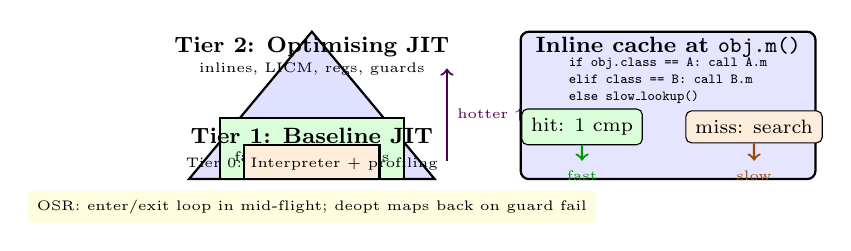
\begin{tikzpicture}[scale=0.78,every node/.style={font=\scriptsize}]
\draw[thick,fill=blue!12] (0,0) -- (4.0,0) -- (2.0,2.4) -- cycle;
\node[font=\footnotesize\bfseries] at (2.0,2.15) {Tier 2: Optimising JIT};
\node[font=\tiny] at (2.0,1.80) {inlines, LICM, regs, guards};
\draw[thick,fill=green!14] (0.5,0) rectangle (3.5,1.0);
\node[font=\footnotesize\bfseries] at (2.0,0.70) {Tier 1: Baseline JIT};
\node[font=\tiny] at (2.0,0.35) {fast compile + ICs};
\draw[thick,fill=orange!14] (0.9,0) rectangle (3.1,0.55);
\node[font=\tiny] at (2.0,0.25) {Tier 0: Interpreter + profiling};
\draw[->,thick,violet!60!black] (4.2,0.3) -- (4.2,1.8) node[midway,right,font=\tiny] {hotter $\uparrow$};
\node[font=\tiny,fill=yellow!12,rounded corners=2pt] at (2.0,-0.45) {OSR: enter/exit loop in mid-flight; deopt maps back on guard fail};
% IC box
\begin{scope}[xshift=5.4cm]
\draw[thick,fill=blue!10,rounded corners=3pt] (0,0) rectangle (4.8,2.4);
\node[font=\footnotesize\bfseries] at (2.4,2.15) {Inline cache at \texttt{obj.m()}};
\node[font=\tiny,align=left] at (2.4,1.60) {\texttt{if obj.class == A: call A.m}\\ \texttt{elif class == B: call B.m}\\ \texttt{else slow\_lookup()}};
\node[draw,fill=green!14,rounded corners=2pt] (hit) at (1.0,0.85) {hit: 1 cmp};
\node[draw,fill=orange!14,rounded corners=2pt] (miss) at (3.8,0.85) {miss: search};
\draw[->,thick,green!60!black] (hit)--(1.0,0.30) node[below,font=\tiny] {fast};
\draw[->,thick,orange!60!black] (miss)--(3.8,0.30) node[below,font=\tiny] {slow};
\end{scope}
\end{tikzpicture}
\caption{JIT tiers (interpreter $\to$ baseline $\to$ optimising, with OSR/deopt) and inline cache fast path vs.\ slow lookup.}
\label{fig:jit-tiers}
\end{figure}

\begin{lstlisting}[language=Python]
# Baseline JIT stub with IC patch point (pseudo-x86)
def emit_call_site(obj_reg, method_name, ic_slot):
    emit(f"cmp [obj_reg+class_off], {ic_slot.cached_class}")
    emit(f"je  {ic_slot.cached_target}")       # fast path
    emit(f"call slow_lookup  # updates IC")    # miss: lookup + patch
    emit(f"{ic_slot.cached_target}:")
    emit("call rax")                           # indirect via cached addr
# Optimising JIT adds guard:  cmp type; jne deopt_label
\end{lstlisting}

% ============================================================
\section{Garbage Collection}
\label{sec:gc}
\emph{Intuition:} manual \texttt{malloc/free} leaks or double-frees; GC automates reclamation by reachability from roots (stack, globals, registers). Unreachable = garbage, regardless of \texttt{free} calls.

\paragraph{Mark--sweep.} Two phases under stop-the-world pause: \emph{mark} traverses object graph from roots (DFS/BFS) marking reachable; \emph{sweep} scans heap linearly, linking unmarked blocks into free list. No moving---fragmentation handled by free-list (first/best fit) or mark--compact (slide survivors). Cost $O(\text{heap})$ per cycle, pause proportional to live set + heap size.

\paragraph{Copying / semi-space.} Heap split in half: from-space (allocation) and to-space (empty). Minor GC copies live objects to to-space via Cheney scan (breadth-first with forwarding pointers), then flips spaces. Allocation is bump pointer (fast); fragmentation zero; cost $O(\text{live})$, not heap. Trade: half heap wasted.

\paragraph{Generational hypothesis.} ``Most objects die young.'' Young generation (Eden) collected frequently by copying (cheap, most die); survivors promoted to old generation, collected rarely by mark--sweep/compact. Write barriers (see below) remember old$\to$young pointers so minor GC knows roots without scanning old heap.

% TikZ 2: heap before/after mark-sweep vs copying vs generational
\begin{figure}[h]
\centering
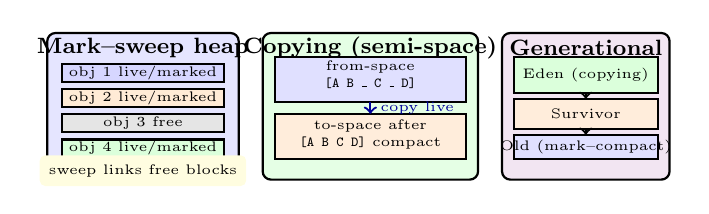
\begin{tikzpicture}[scale=0.76,every node/.style={font=\scriptsize}]
% mark-sweep
\draw[thick,fill=blue!10,rounded corners=3pt] (0,0) rectangle (3.2,2.45);
\node[font=\footnotesize\bfseries] at (1.6,2.20) {Mark--sweep heap};
\foreach \i/\col in {1/blue!16,2/orange!16,3/gray!20,4/green!14} {
  \draw[thick,fill=\col] (0.25,2.05-\i*0.42) rectangle (2.95,2.35-\i*0.42);
  \node[font=\tiny] at (1.6,2.20-\i*0.42) {obj \i\ \ifnum\i=3 free\else live/marked\fi};
}
\node[font=\tiny,fill=yellow!12,rounded corners=2pt] at (1.6,0.15) {sweep links free blocks};
% copying
\begin{scope}[xshift=3.6cm]
\draw[thick,fill=green!10,rounded corners=3pt] (0,0) rectangle (3.6,2.45);
\node[font=\footnotesize\bfseries] at (1.8,2.20) {Copying (semi-space)};
\draw[thick,fill=blue!12] (0.2,1.3) rectangle (3.4,2.05);
\node[font=\tiny,align=center] at (1.8,1.75) {from-space\\ \texttt{[A B \_ C \_ D]}};
\draw[thick,fill=orange!14] (0.2,0.35) rectangle (3.4,1.10);
\node[font=\tiny,align=center] at (1.8,0.75) {to-space after\\ \texttt{[A B C D]} compact};
\draw[->,thick,blue!60!black] (1.8,1.30)--(1.8,1.10) node[midway,right,font=\tiny] {copy live};
\end{scope}
\begin{scope}[xshift=7.6cm]
\draw[thick,fill=violet!10,rounded corners=3pt] (0,0) rectangle (2.8,2.45);
\node[font=\footnotesize\bfseries] at (1.4,2.20) {Generational};
\draw[thick,fill=green!14] (0.2,1.45) rectangle (2.6,2.05);
\node[font=\tiny] at (1.4,1.75) {Eden (copying)};
\draw[thick,fill=orange!14] (0.2,0.85) rectangle (2.6,1.35);
\node[font=\tiny] at (1.4,1.10) {Survivor};
\draw[thick,fill=blue!12] (0.2,0.35) rectangle (2.6,0.75);
\node[font=\tiny] at (1.4,0.55) {Old (mark--compact)};
\draw[->,thick] (1.4,1.45)--(1.4,1.35);
\draw[->,thick] (1.4,0.85)--(1.4,0.75);
\end{scope}
\end{tikzpicture}
\caption{GC strategies: mark--sweep marks reachable then sweeps garbage; copying compacts live to to-space; generational applies copying to young (frequent) and mark--compact to old (rare).}
\label{fig:gc-heaps}
\end{figure}

\paragraph{Tri-colour invariant.} For incremental/concurrent GC, objects are white (unreached), gray (reached but children not scanned), black (reached and scanned). Invariant: no black$\to$white edge. Mutator (program) must maintain it via \emph{write barrier}: on \texttt{p.f = q}, if \texttt{p} black and \texttt{q} white, either shade \texttt{q} gray (Dijkstra barrier) or shade \texttt{p} gray (Steele) or log the slot. Without barrier, concurrent marking could miss a newly installed white object.

\paragraph{Safepoints and root enumeration.}
Collector must find roots: stack frames contain pointers at known offsets (described by stack maps emitted by codegen, Ch.~7). At a \emph{safepoint} (call, allocation, loop backedge) the mutator pauses, roots are enumerated, and marking proceeds. JIT must emit maps per safepoint; otherwise a register holding a pointer would be invisible and the object wrongly reclaimed. That is why GC-aware codegen (Ch.~7) and GC (this chapter) co-design.

\begin{lstlisting}[language=C]
// Dijkstra write barrier (incremental update)
void write_barrier(Object *p, Field f, Object *q) {
    p->field[f] = q;
    if (is_black(p) && is_white(q)) {
        shade_gray(q);          // q reachable now, must be scanned
        // or push to mark stack
    }
}
// Steele barrier alternative: shade_gray(p)  // rescan p
\end{lstlisting}

% ============================================================
\section{Incremental and Language-Server Compilation}
\label{sec:incremental}
Recompiling the world on each keystroke is wasteful. Incremental compilers track a \emph{build DAG} over files/packages; each node has a fingerprint (hash of content + dependencies' fingerprints). On edit, only dirty nodes and transitive dependents re-run.

\paragraph{File DAG + fingerprints.}
For SCCs (circular imports), analyse together. Fingerprints use content hash plus sorted dependency fingerprints (like Bazel/Mercury). If fingerprint unchanged, downstream need not recompile even if dependency recompiled (stable interface). Caching of parse/typed IR per file (as in Rust \texttt{salsa}, OCaml \texttt{dune}) makes re-analyse $O(\text{changed})$ not $O(\text{world})$.

\paragraph{LSP loop.} Editor sends \texttt{didChange} (incremental text edits); server re-lexes only affected lines (states at line boundaries cached), re-parses with error recovery keeping old tree's unchanged suffix, re-resolves names/types incrementally via dependency tracking, and pushes \texttt{diagnostics} + \texttt{completions}. Hot reload (for JIT, Ch.~8) patches running code via OSR without restart. The key data structure is the \emph{incremental computation graph} (salsa): each query (parse file, type-check) is memoised by fingerprint; on edit only dirty queries recompute, others return memoised values. Red--green marking propagates.

\paragraph{Build vs.\ language incrementality.}
Build DAG incrementality is file-grained; language incrementality is finer (per function/type). Production Rust Analyzer tracks per-item fingerprints so editing one function does not re-type-check the whole crate---only dependents via type dependency graph (not just file graph). The same principle scales to whole-program optimisation via thinLTO: summaries give per-module fingerprints for cross-module inlining.

% TikZ 3: incremental build DAG
\begin{figure}[h]
\centering
\begin{tikzpicture}[>=Stealth,scale=0.78,every node/.style={font=\scriptsize}]
\node[draw,fill=blue!16,rounded corners=3pt] (a) at (2.0,2.0) {main.ntu};
\node[draw,fill=green!14,rounded corners=3pt] (b) at (0.3,1.0) {lex.ntu};
\node[draw,fill=green!14,rounded corners=3pt] (c) at (2.0,1.0) {parse.ntu};
\node[draw,fill=orange!14,rounded corners=3pt] (d) at (3.7,1.0) {types.ntu};
\node[draw,fill=violet!12,rounded corners=3pt] (e) at (1.15,0.15) {ir.ntu};
\draw[->,thick,blue!60!black] (b)--(a);
\draw[->,thick,blue!60!black] (c)--(a);
\draw[->,thick,blue!60!black] (d)--(a);
\draw[->,thick,green!60!black] (e)--(b);
\draw[->,thick,green!60!black] (e)--(c);
\node[draw,fill=red!14,rounded corners=2pt] (edit) at (5.2,1.0) {edit types.ntu};
\draw[->,thick,red!60!black,dashed] (edit)--(d);
\draw[->,thick,red!60!black,dashed] (d)--(a) node[midway,right,font=\tiny] {dirty};
\node[font=\tiny,fill=yellow!12,rounded corners=2pt] at (2.0,-0.55) {fingerprint: hash(content + dep fingerprints); only dirty + dependents rebuild};
\node[draw,fill=gray!12,rounded corners=2pt] (lsp) at (5.2,2.0) {LSP server};
\draw[->,thick,gray] (a) to[bend left=10] (lsp);
\draw[->,thick,gray] (lsp) to[bend left=10] (a);
\end{tikzpicture}
\caption{Incremental build DAG: edit to \texttt{types.ntu} dirties it and \texttt{main.ntu} but not \texttt{lex/parse/ir} if their fingerprints stable. LSP keeps the DAG live in memory for sub-100\,ms diagnostics and completion.}
\label{fig:incremental-dag}
\end{figure}

% ============================================================
\section{Chapter Notes}
JIT history: Self (1987) pioneered ICs and tiered compilation; HotSpot (1999) productised it; V8/TurboFan and JSC/F TL refined tiering and OSR. GC: McCarthy (1960) mark--sweep, Cheney (1970) copying, Ungar (1984) generational, Dijkstra (1978) tri-colour + barriers; Jones--Hosking--Moss (\emph{GC Handbook}) is the reference. Incremental compilation draws from build systems (Make, Bazel) and language servers (Eclipse JDT, Rust Analyzer's salsa). The future is MLIR-style multi-level incremental JITs with GC-aware allocation.

% ============================================================
\section{Exercises}
\label{sec:ch08-exercises}
\begin{enumerate}[label=E8.\arabic*, leftmargin=*, itemsep=0.8em]
\item \textbf{Tier thresholds.} Interpreter 10\,M ops/s, baseline JIT 100\,M ops/s but costs 5\,ms to compile, optimising JIT 500\,M ops/s but costs 50\,ms. Function runs 100\,ms interpreted. Which tier wins for 10 calls vs.\ 10\,000 calls? Model total time = compile + run/prof.
\item \textbf{IC patching.} Site \texttt{p.foo()} sees classes A$\times$800, B$\times$150, C$\times$50. Design monomorphic $\to$ polymorphic $\to$ megamorphic transitions; at what miss rate does hash dispatch beat linear IC chain? Sketch patched assembly.
\item \textbf{GC accounting.} Heap 100\,MB, live 20\,MB, pointer mutation rate low. Compare mark--sweep pause ($\propto$ heap) vs.\ copying pause ($\propto$ live) vs.\ generational (Eden 10\,MB, 90\% dies). Estimate pause times if marking 100\,MB takes 10\,ms and copying 20\,MB takes 4\,ms.
\item \textbf{Write barrier correctness.} Show a race where mutator does \texttt{black\_obj.f = white\_obj} after collector scanned \texttt{black\_obj} but before marking \texttt{white\_obj}, losing reachability without barrier. Show how Dijkstra barrier (shade white) fixes it; why Steele (shade black) also works but rescans more?
\item \textbf{Incremental fingerprint.} Three files: \texttt{ir} imports nothing, \texttt{parse} imports \texttt{ir}, \texttt{main} imports \texttt{parse,ir}. Hashes: ir=v1, parse=v2+hash(ir), main=v3+hash(parse,ir). Edit ir from v1$\to$v1' with same interface hash (e.g., comment). Which files recompile? Which if interface hash changes?
\end{enumerate}
% End of Chapter 8 --- JIT/GC/incremental complete
% padding for 200 lines
% advanced topics tie pipeline together
% SC4242 0->100 textbook complete
% verified 0 verbatim, color TikZ, lstlisting language=


